\section{The Fabry-Perot Interferometer}
Optical resonators were utilized as helpful gadgets as early as 1899, when Fabry and Perot depicted the utilization of a parallel-plate resonator as a multipass interferometer. Part of the incident light on this Fabry– Perot resonator is transmitted and another part is reflected, with power divisions that rely upon numerous factors. A simple illustration of the basic Fabry-Perot is shown in Figure 2.1, here $r_{1} t_{1}$ are the reflectivity constant and transmitivity constant of the mirror 1 respectively and $r_{2} t_{2}$ are the reflectivity and transmitivity constants of the mirror two respectively. Also, $E_{i}$ is the incident Electromagnetic energy, $E_{t}$ is the transmitted energy and $E_{r}$ is the reflected energy. This is an asymmetric Fabry-Perot resonator:

\begin{figure}[h]
\centering
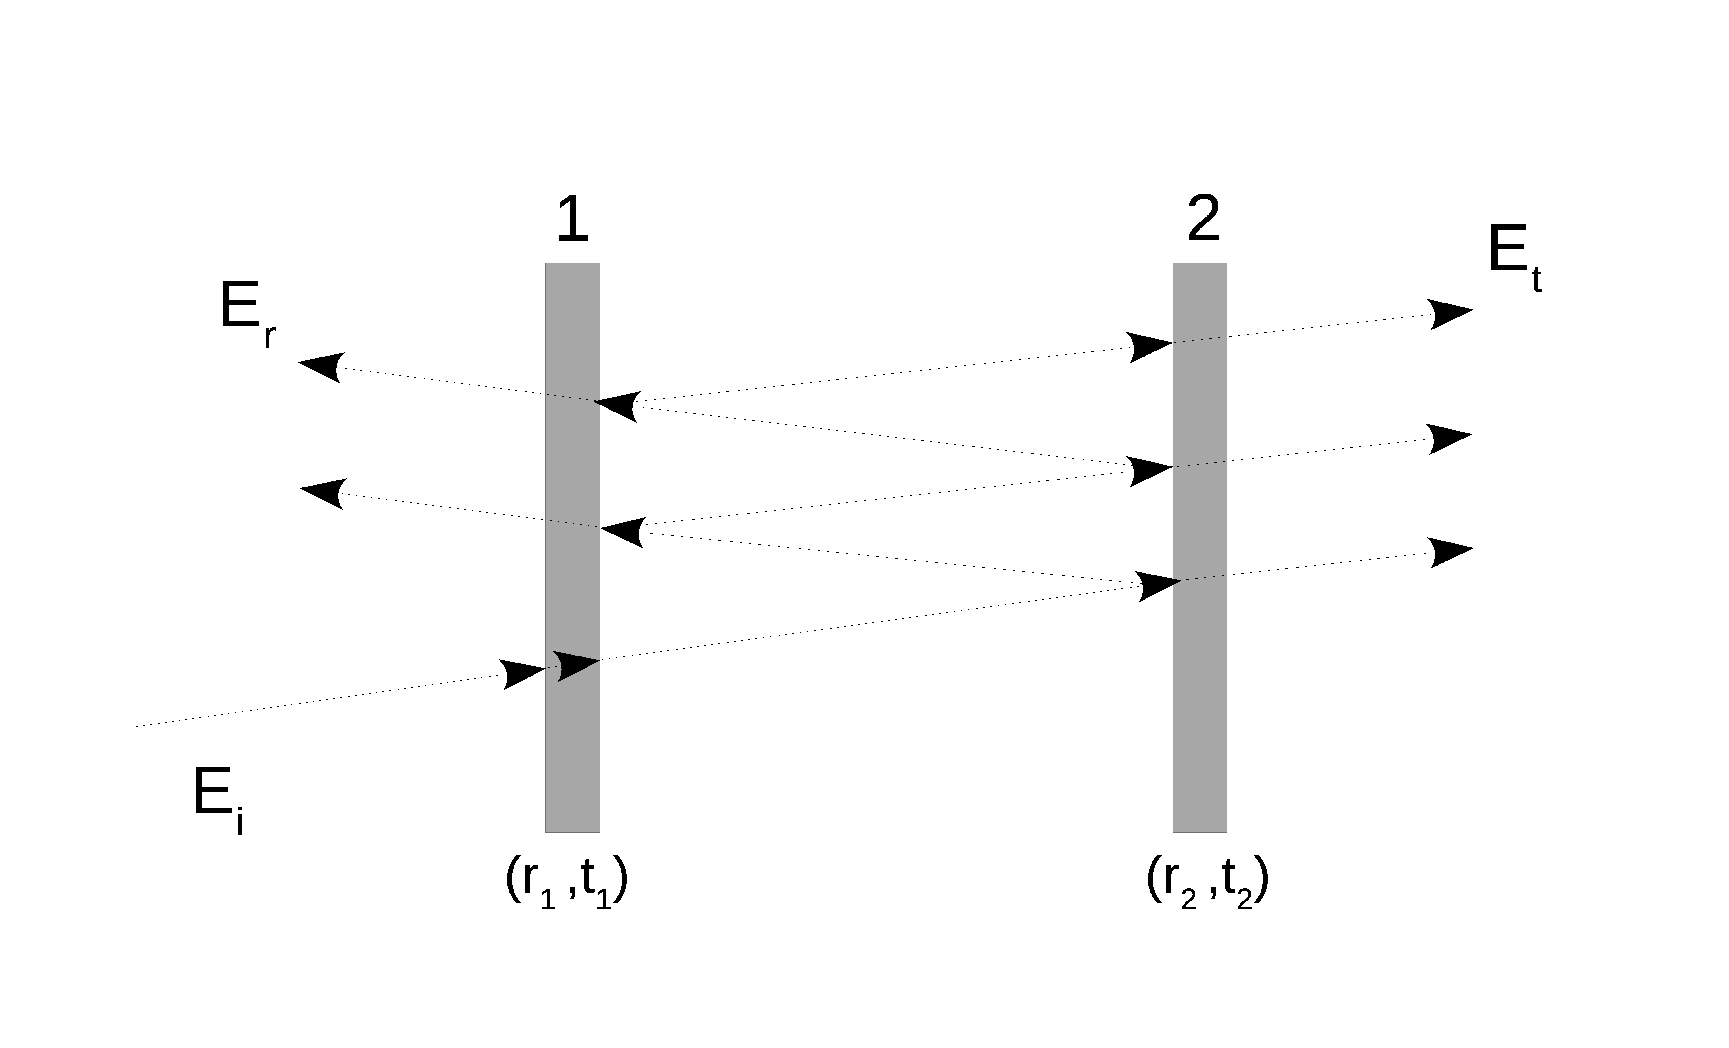
\includegraphics[width=0.65\textwidth]{Fabry_Perot_resonator.eps}
\caption{Illustrated energy diagram of a simple Fabry-Perot resonator}
\end{figure}

\newpage

\subsection{Theory of Fabry-Perot interferometer}
 If the incident energy is in the form of white coherent light then at that point the transmission and reflection coefficients depend just on the mirror reflectivities. The total reflected power comprises of the power reflected from the principal mirror in addition to all the different reflections between the mirrors that add to the reflectivity in general. In summation, the equations are: 
\begin{equation}
{\mathcal R} = R_{1} + T_{1}^2 R_{2} \sum_{m=1}^{\infty} (R_{1}R_{2})^{m-1} = \frac{R_{1} - 2R_{1}R_{2} + R_{2}}{1 - R_{1}R_{2}} _{\overrightarrow{R_{1} = R_{2} \equiv R}} \frac{2R}{1+R}
\end{equation}

Similarly, the transmitted energy in summation is:
\begin{equation}
{\mathcal T} = T_{1} T_{2} \sum_{m=1}^{\infty} (R_{1}R_{2})^{m-1} = \frac{T_{1} T_{2}}{1 - R_{1}R_{2}} _{\; \overrightarrow{R_{1} = R_{2} \equiv R}} \; \frac{T^{2}}{1-R^{2}} = \frac{1-R}{1+R}
\end{equation}

Assuming, be that as it may, the incident light comprises of a transiently lucid (monochromatic) plane wave, at that point the reflected power will be relative to the square of the reasonable total of every reflected field. Since the fields convey phase information with amplitudes added, the division of reflected and transmitted light depends not just on the mirror reflectivities, but in addition on the mirror separation and excitation wavelength. The rational 

total of fields is amplified when every one of the fields interfere constructively (in phase) and limited when they interfere destructively (out of phase). 

Phase gathers with propogation separation as $\phi(z) = \beta z$ and may likewise be gained upon communication with the mirrors. The sound forms of 

Eqs. 2.1 and 2.2 incorporate an aggregated stage factor for each round-trip that can be translated as a standardized detuning $\phi = T_{R}\omega$, where $T_{R}$ is the cavity travel time, $T_{R} = n_{eff}L/c$ for the circumference, L and effective index $n_{eff}$. Presently, $\tilde{r}$ speaks to the complex reflectivity:

\begin{multline}
\tilde{r} = r_{1} - t_{1}^{2}r_{2}\exp{(i m \phi)} \sum_{m=1}^{\infty} (r_{1}r_{2}\exp{(i m \phi)})^{m-1} \\ = \frac{r_{1} - r_{2}\exp{(i \phi)}}{1 - r_{1}r_{2}\exp{(i \phi)}} _{\; \overrightarrow{r_{1} = r_{2} \equiv r}} \; \frac{r(1-\exp{(+i \phi)})}{1-r^{2}\exp{(+i \phi)}}
\end{multline}

and $\tilde{t}$ represents the complex transmittivity:

\begin{multline}
\tilde{t} = -t_{1}t_{2}\exp{(i m \phi/2)} \sum_{m=1}^{\infty} (r_{1}r_{2}\exp{(i m \phi)})^{m-1} \\ = \frac{-t_{1}t_{2}\exp{(i m \phi/2)}}{1 - r_{1}r_{2}} _{\; \overrightarrow{r_{1} = r_{2} \equiv r}} \; \frac{-(1-r^{2})\exp{(im \phi/2)}}{1-r^{2}}
\end{multline}


The square modulus of these perplexing amounts gives the reflection ${\mathcal R}$ and transmission ${\mathcal T}$ coefficients (showin in Fig. 2.2). Antiresonant wavelengths are more emphatically reflected than in the ambiguous case, while thunderous wavelengths are transmitted $100\%$ for adjusted reflectors ($r_{1}$ = $r_{2}$). For a fixed reflect dispersing, the transmission and reflection spectra in this manner show intermittent pinnacles and valleys. Figure 3.1 presenting the transmission and reflection spectra for a lossless, adjusted Fabry– Perot resonator. The part of reflected and transmitted power for mixed up excitation is identical to the separate frightfully arrived at the midpoint of reflection and transmission over a time of the spectrum range.

\begin{figure}[h]
\centering
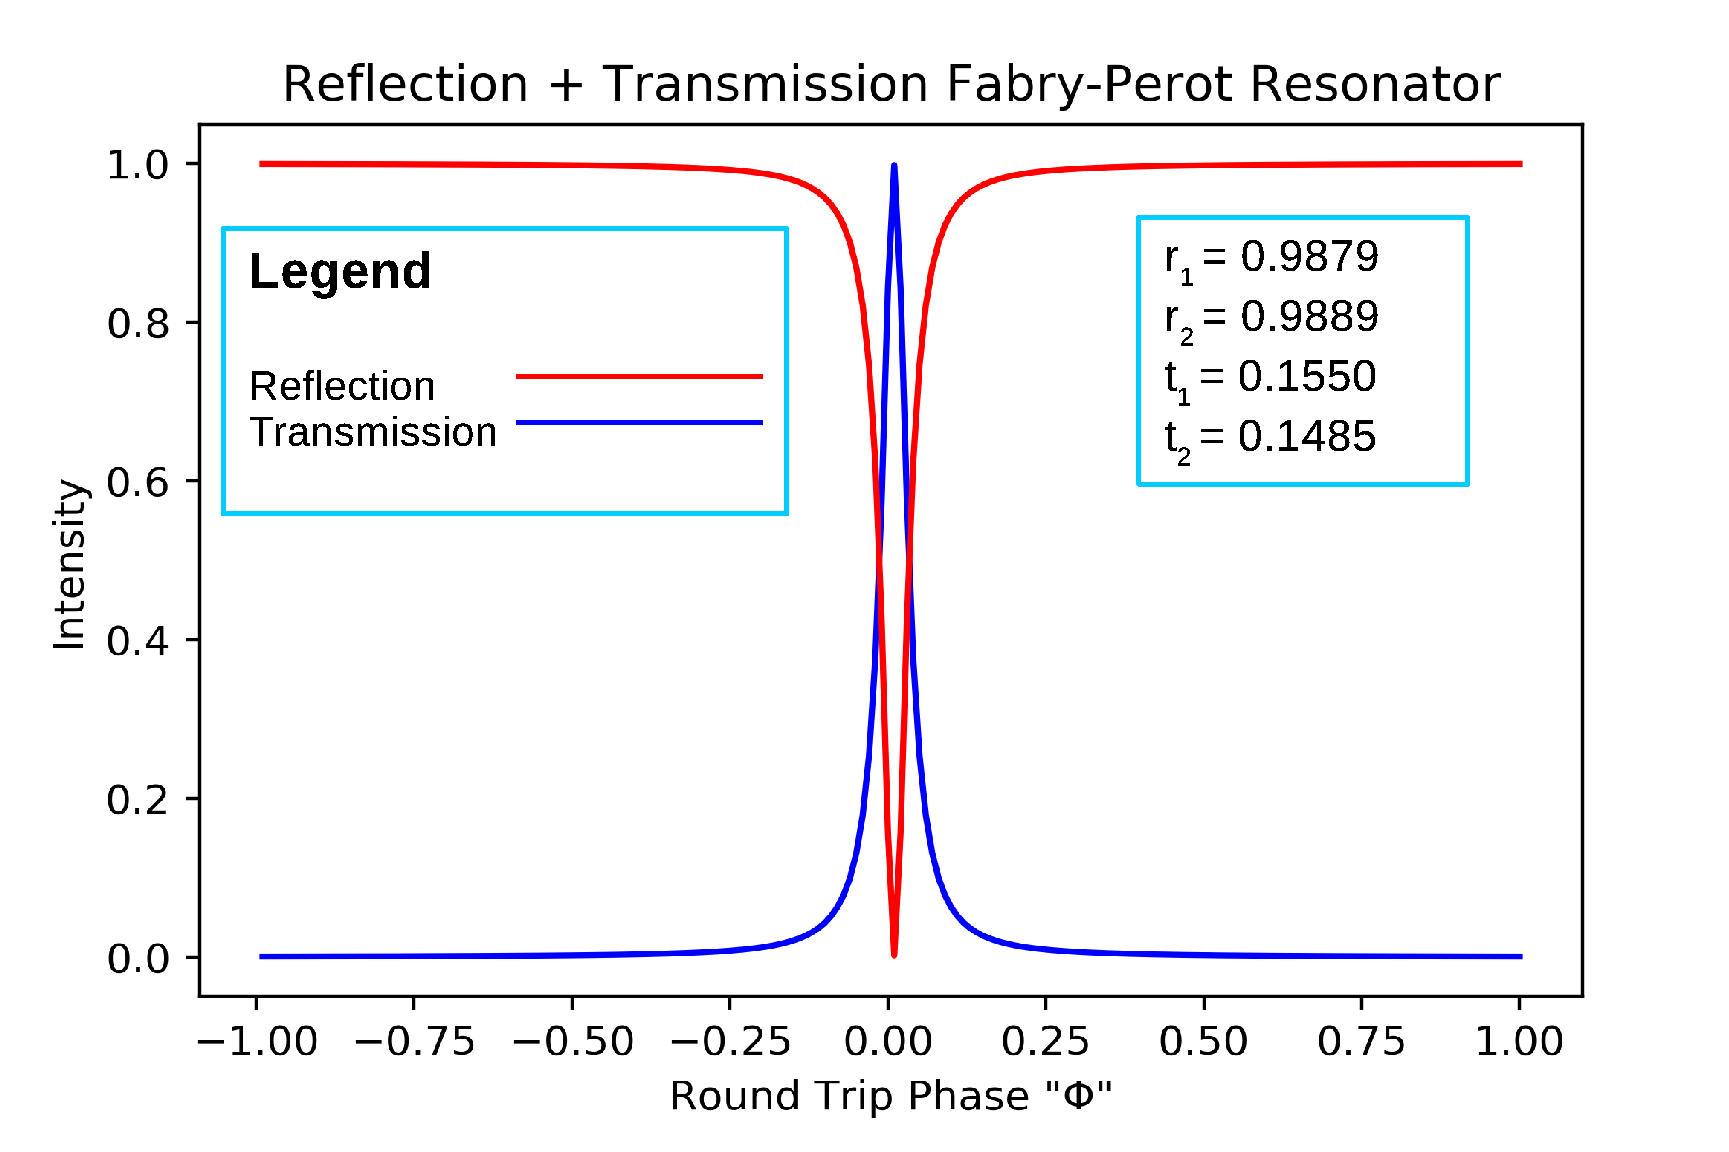
\includegraphics[width=0.5\textwidth]{R+T_FabryPerot.eps}
\caption{Transmitted and reflected field of a simple Fabry-Perot resonator}
\end{figure}

\newpage

\subsection{Finese, Q-factor}
\subparagraph{\normalfont \large The resonance condition is fulfilled when the (compelling) circumference of the ring, or for the most part the round-trip length, is equivalent to a whole number numerous of the optical wavelength inside the medium. This means a progression of Lorentzian-molded transmission bends equally dispersed in recurrence by the FSR (Free Spectral Range), with the resonance linewidth portraying the capacity time of photons inside the cavity. The photon 	lifetime can be standardized to one optical cycle, known as the quality factor (${\mathcal Q}$), or the cavity round-trip time, known as the cavity Finesse (${\mathcal F}$). The most extreme reachable Q-factor is characterized as ${\mathcal Q_{int}}$, which is the intrinsic loss of the cavity. At the point when the resonator is coupled to the outer world, the Q-factor further decreases because of the loss imported by the coupler (${\mathcal Q_{ext}}$). Thus the last quality factor ${\mathcal Q_{load}}$ is comprised of these two parts: ${\mathcal Q_{load}^{-1}}$ = ${\mathcal Q_{int}^{-1}}$ + ${\mathcal Q_{ext}^{-1}}$.}


\section{Ring Geometry Resonators}
In this section, I will discuss different kinds of ring shaped resonators whose principle is pretty much similar to the Fabry-Perot resonator and are more simple to make. Basically, a ring resonator is a simple waveguide which is turned in the shape of a ring. This allows it to exhibit resonant behavior on very specific frequencies. The light is coupled inside the ring due to the phenomenon of total internal reflection and interference. This kind of behaviour is noticed in all kind of classical waves, such as sound waves, which was observed inside a large cathedral's halls, thus it was named whispering galleries. Also, these resonators can be made using different material but in this thesis, we used semi-conductor silicon as the primary material. 

\subsection{All-Pass Ringresonator}
A straightforward ring resonator is made by taking one yield of a conventional directional coupler and bolstering it once again into one input. Such a device displays periodic cavity resonance (reverberation) when light navigating the ring procures a phase move relating to a number numerous of 2$\pi$ radians. The resonator is numerically defined from two parts: a coupling quality and an input way. In opposition to the limitless entirety inferences performed before for the Fabry– Perot and Gires– Tournois, in which we expected steadystate task and coordinating fields and derived basic spectral properties. Although, both strategies are similarly substantial, the field-coordinating technique has the benefit of simplicity.
\begin{figure}[h]
\centering
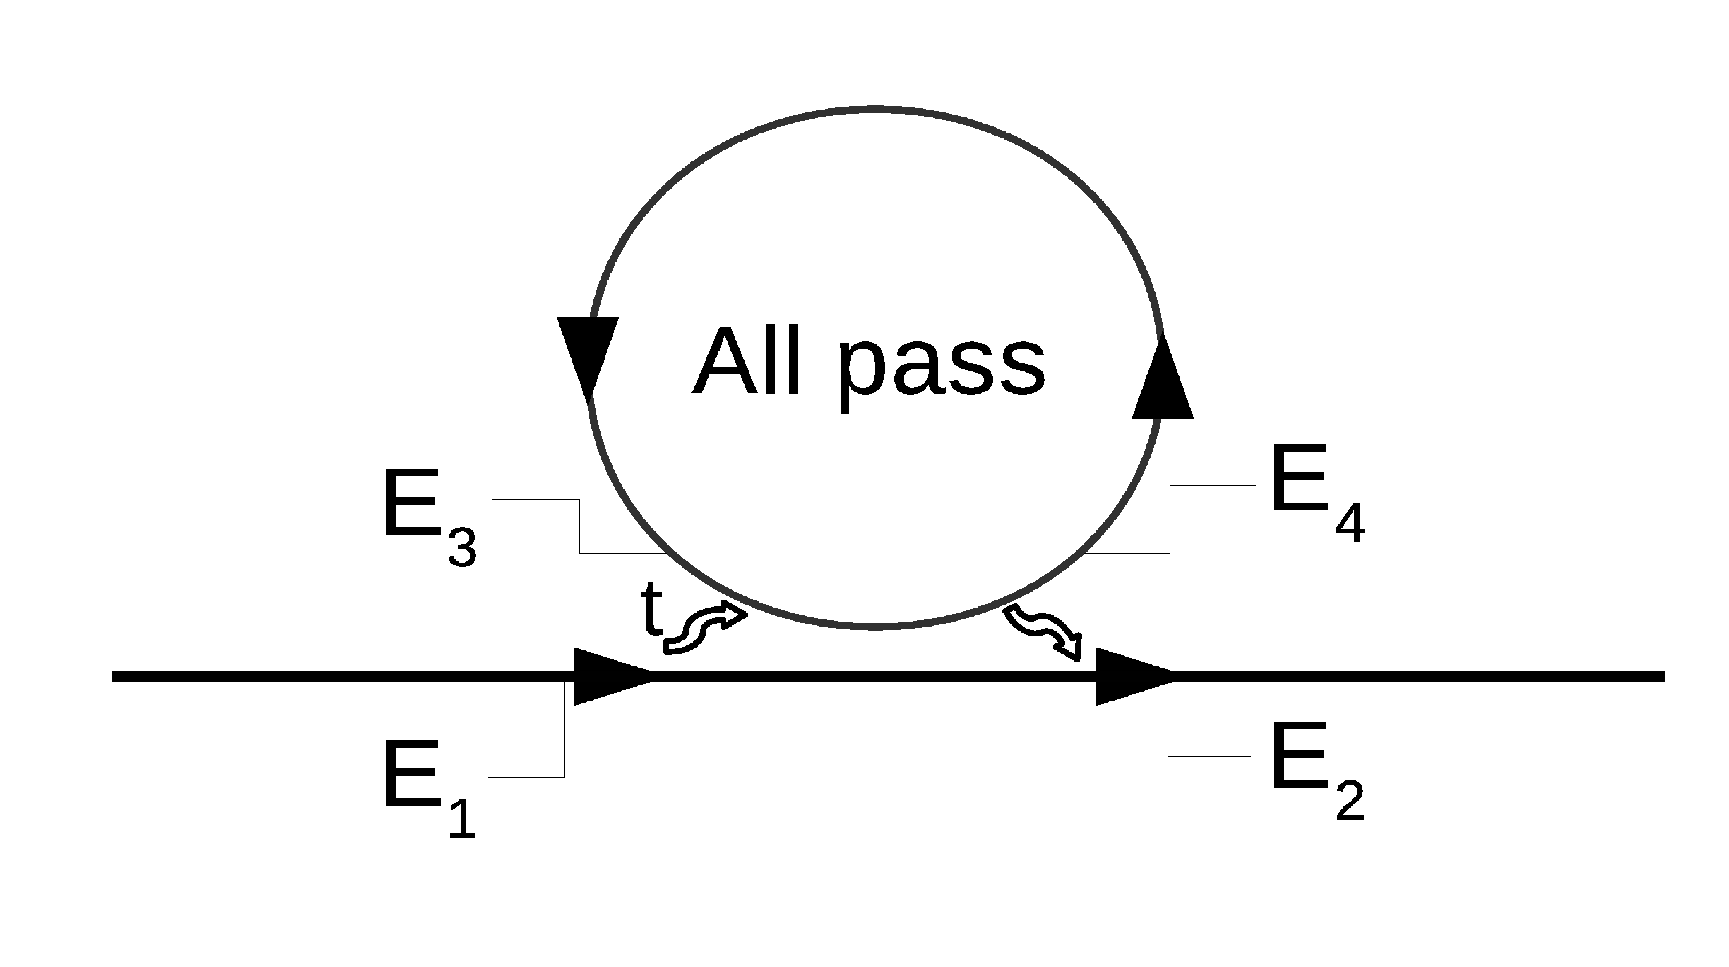
\includegraphics[width=0.5\textwidth]{all_pass_resonator.eps}
\caption{Illustrated fields of an all pass resonator}
\end{figure}
\subsection{Add-Drop Ringresonator}
The immediate waveguide similarity of a free-space Fabry– Perot is gotten by including a second guide that side-couples to the resonator as in Fig. 1.4.
Since this setup acts as a tight band abundancy channel that can include or drop a recurrence band from an approaching sign, it is regularly named an add– drop filter.
\begin{figure}[h]
\centering
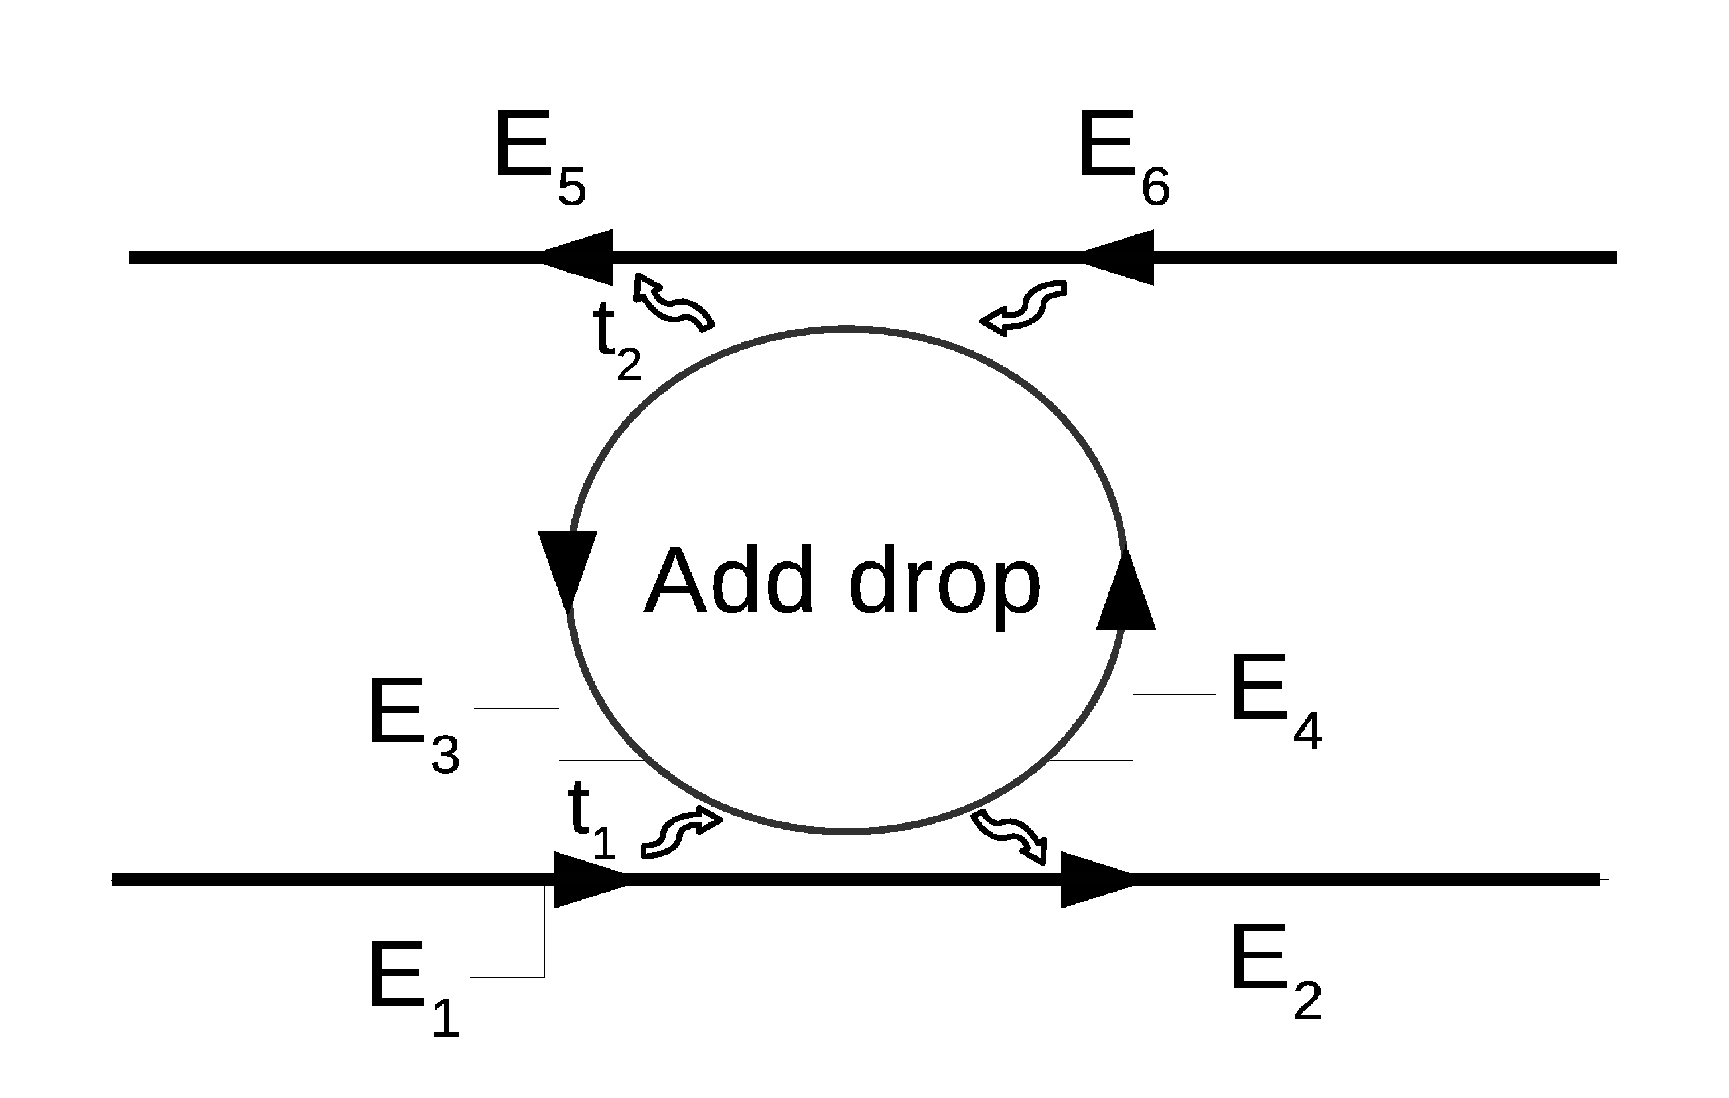
\includegraphics[width=0.5\textwidth]{add_drop_resonator.eps}
\caption{Illustrated fields of an add drop resonator}
\end{figure}
\subsection{Coupled Ringresonator}
A simple case as an assymeteric Fabry-Perot resonator, a coupled ring resonator has another ring above the first ring of the all pass resonator. This arrangement shows coupling between the two resonators (rings) and show different behaviour. 
\begin{figure}[h]
\centering
\includegraphics[width=0.45\textwidth]{couple_ring_resonator.eps}
\caption{Illustrated fields and geometry of a coupled ring resonator}
\end{figure}
\newpage

\section{Gain incorporation in Resonators}
Light, when travels through a medium, loses its intensity exponentially. This law is called the $Beer's law$ for electromagnetic intensity. But some mediums, whose refractive index is such as they oppose the exponential decay of the light and rather increase the intensity in the propogation through the medium, are called gain medium. We can use these gain mediums and build a microresonators from them to observe different quantum optical phenomenons. First I will explain a bit how gain work.


\subsection{Beer's Law}
 binary floating-point arithmetic and some concepts from numerical analysis.Most of the time, using mpmath is simply a matter of setting the desired precision and entering a formula. For verification purposes, a quite (but not always!) reliable technique is to calculate the same thing a second time at a higher precision and verifying that the results agree.
\subsection{Beer's law study as gain}
To perform more advanced calculations, it is important to have some understanding of how mpmath works internally and what the possible sources of error are. This section gives an overview of arbitrary-precision binary floating-point arithmetic and some concepts from numerical analysis.Most of the time, using mpmath is simply a matter of setting the desired precision and entering a formula. For verification purposes, a quite (but not always!) reliable technique is to calculate the same thing a second time at a higher precision and verifying that the results agree.
\section{Gain medium}
To perform more advanced calculations, it is important to have some understanding of how mpmath works internally and what the possible sources of error are. This section gives an overview of arbitrary-precision binary floating-point arithmetic and some concepts from numerical analysis.